\documentclass{article}

\usepackage{amsmath,amssymb,graphicx,caption,subcaption}
\setlength{\parindent}{0cm}
\setlength{\parskip}{12pt}
\usepackage[margin=1in]{geometry}

\newcommand{\tb}{\texttt{'trainBust'}}
\newcommand{\s}{\vec{\sigma}}
\renewcommand{\d}{\vec{\delta}}
\newcommand{\e}{\varepsilon}
\newcommand{\grad}{\bigtriangledown}

\begin{document}

This document pertians to the function \tb

\section{definitions}
For the purposes to follow, \tb has the following properties:
\begin{enumerate}
\item Performs 1 step of an implicit-qr algorithm 
  (using householder projections) on a Hessenberg matrix $H$
\item extracts a series of $m$ numbers upon completion, to be referred to as outputs.
\item takes an input of $s$ shifts to use in the implicit-qr algorithm. to be referred to as inputs.
\item capable of taking an input of size $s \times d$ to represent
  $d$ seeds for automatic differentiation
\item capable of returning the resulting $d \times 2m$ outputs of the automatic differentiation
\end{enumerate}

For those interested, the extraction of the $2 \cdot m$ numbers is performed by
performing a schur decomposition of a submatrix embedded within the larger matrix.
This schur decomposition results in a spike (or 2 spikes if perfomed in the middle),
the values of which are the $m$ numbers.

In the framework considering the shifts as inputs and the spikes as outputs,
we can view this algorith as performing the following transformation
\[
  T:\mathbb{C}^s \to \mathbb{C}^m
\]
Let the shifts be $\s \in \mathbb{C}^s$ and the spikes be $\vec{m} \in \mathbb{C}^m$.
Then we can define the Jacobian as 
\[
  J \in \mathbb{C}^{s \times m} \\
  J_{i,j} = \dfrac{\partial T_i }{\partial \s_j}
\]
Where $T_i$ is the $i^{th}$ output of the function $T$.

If we provide a seed $\d \in \mathbb{C}^s$ to the automatic differentiation provided
in \tb, the end result is equivalent to
\[
  \d \cdot J = [\d \cdot \grad T_i] 
\]
Where the surrounding square brackets indicate that this is a vector
over the free indices (in this case $i$).

\section{Automatic Differentiation Performance}
Note that
\[
  \left.\d \cdot J\right|_{\s} \approx \left[\dfrac{T_i(\s + \e\d) - T_i(\s - \e\d)}{2 \e \| \d \|}\right]
\]
for $\e > 0$.

The following results are based upon using $H \in \mathbb{R}^{100\times100}$, $H$ hessenberg,
chosen by running a hessenberg decomposition on a matrix chosen from randomly from a normal distribution,
$\s$ chosen from a random normal distribution (multiplied by 100), $\d$ was chosen
from a uniform distribution and then normalized, and $s = 8$ ($\e$ is specified below).

Before considering the function $T$, consider the following two processes:
\begin{enumerate}
\item \tb after it has pushed the bulges through the matrix, but before performing a schur
decomposition to create spikes
\item the schur decomposition and its derivative.
\end{enumerate}
Let $B$ be the output of item (1), so $B$ = $B(\s)$.
Furthermore, let $\dot{B}$ represent the derivative of $B$ with respect to 
the normalized direction $\d$.
Then
\[
  \dot{B} \approx \dfrac{B(\s + \e\d) - B(\s)}{\e}
\]
The Schur decomposition is $A = Q'TQ$, where the outputs are $Q$ and $T$.
For the direction $\Delta$, we have that the schur decomposition is
$A + \e \Delta = Q_{\e} T_{\e} Q_{\e}$.
The \texttt{schurAD} fuction calculates $\dot{Q}$ and $\dot{T}$ given $\Delta$.
Thus we have that
\[
  A + \e \Delta \approx (Q + \dot{Q}) (T + \dot{T}) (Q + \dot{Q})'
\]

Thus treating the automatic differentiation result as the exact derivative,
the above finite difference approximations should yield accuracy of $O(\e)$.
The following equations are used to caculate the error:
\[
  er_F(\e) = \dfrac{\|B(\s + \e \d) - (B(\s) + \e \cdot \dot{B})\|_F}{\|B(\s)\|_F}
\]
\[
  er_S(\e) = \dfrac{
    \|(Q + \e \dot{Q}) (T + \e \dot{T}) (Q + \e \dot{Q})' - (A + \e \Delta)\|_F}
    {\|A\|_F}
\]
\[
  er_Q(\e) = \| (Q + \e\dot{Q})(Q + \e\dot{Q})' - I\|_F
\]
Figure \ref{fig:fdErr} shows that the errors are indeed of $O(\e^2)$ (thus accurate
to first order), indicating
that the AD approximation does indeed yield the derivative exact derivative which
the finite difference is approximating.

\begin{figure}[h!]
  \centering
  \begin{minipage}[b]{.5\linewidth}
    \centering
    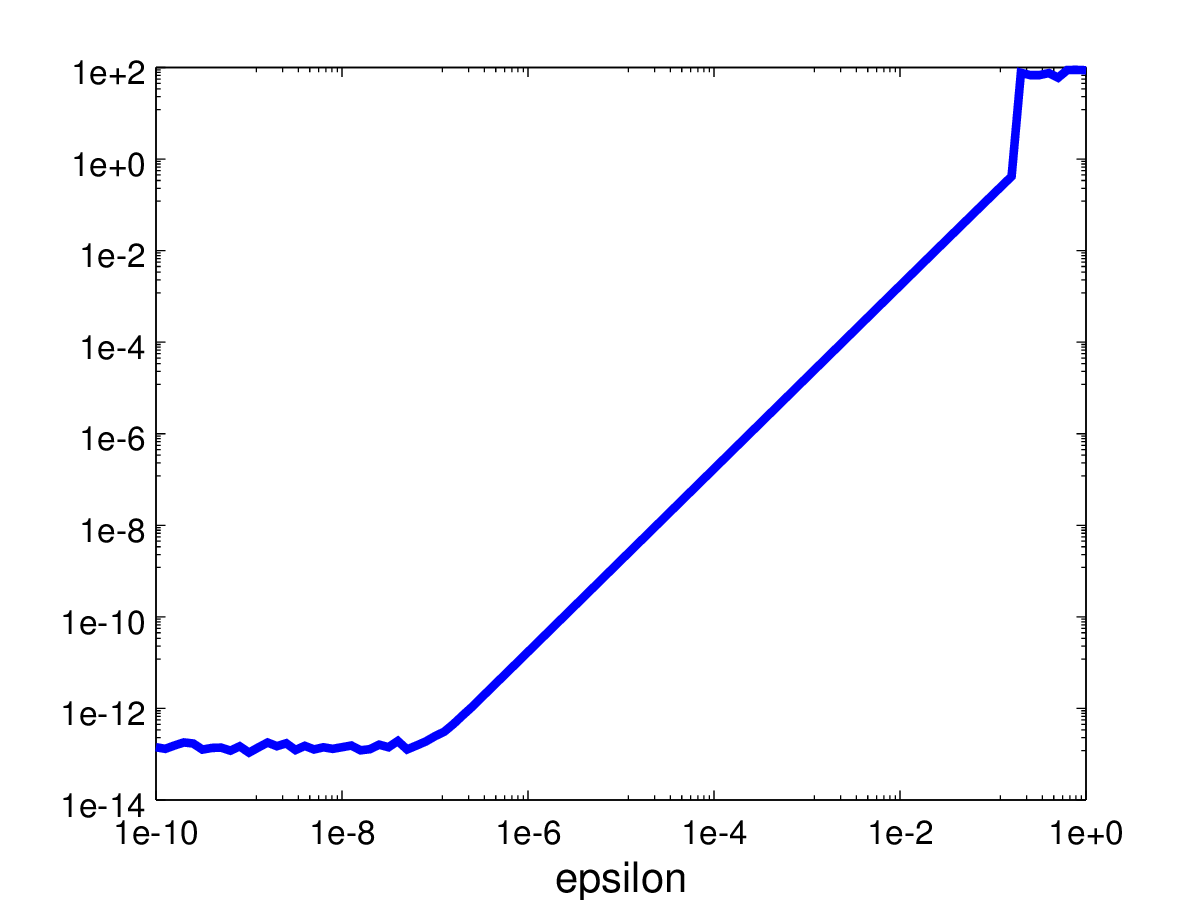
\includegraphics[width=\textwidth]{francisADErr.png}
    \subcaption{$er_F(\e)$}
  \end{minipage}%
  \begin{minipage}[b]{.5\linewidth}
    \centering
    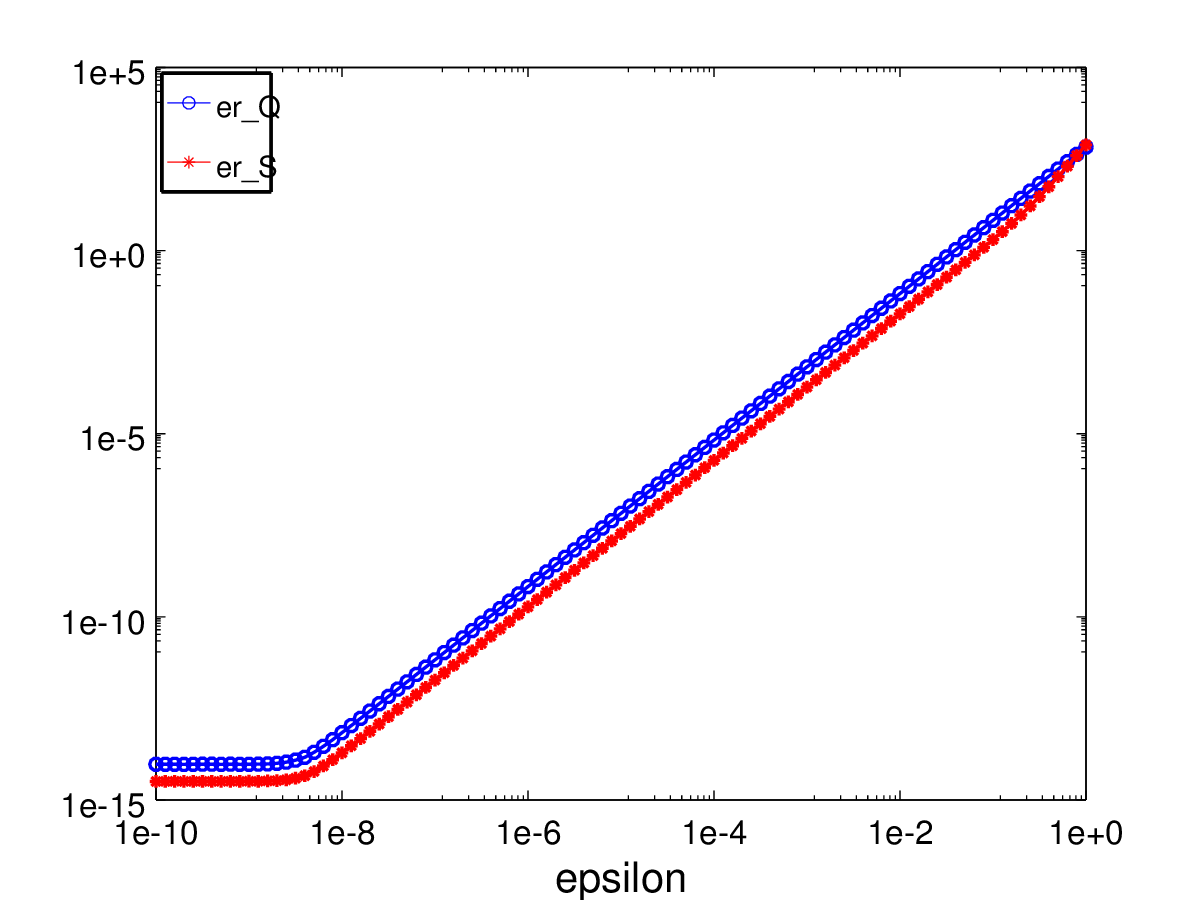
\includegraphics[width=\textwidth]{schurErr.png}
    \subcaption{$er_S(\e)$ and $er_Q(\e)$}
  \end{minipage}

\caption{Finite difference errors}\label{fig:fdErr}
\end{figure}

\section{Completing the process}

Figure \ref{fig:vanErr} shows $er_F$ applied after the schur decomposition
has been used to eliminate the blocks, for 2 different matrices.
The matrices used 10 shifts and were size 100.

\begin{figure}[h!]
  \centering
  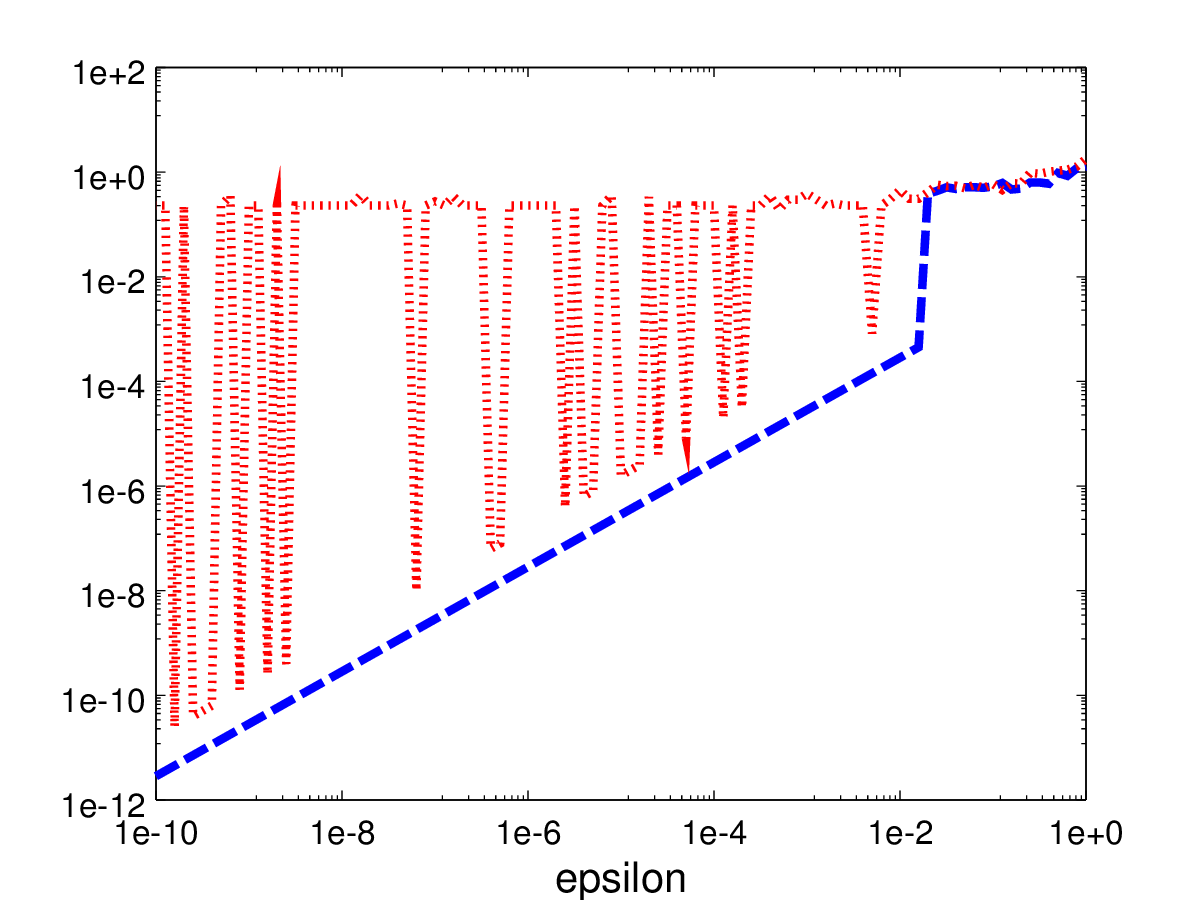
\includegraphics[width=.5\linewidth]{endVanillaError.png}
  \caption{$er_F(\e)$ applied to completed process}\label{fig:vanErr}
\end{figure}

Clearly some matrices break the automatic differentiation as applied/interpreted.
Thid is due to the arbitrary ordering of the eigenvalues which emerge
in the schur decomposition (which can be highly sensitive to perturbations).
To avoid this arbitrariness, the Schur decomposition was sorted using
code published by Jan Brands \cite{srschur}.

%COOL IDEA -> Won't work since must permute entire matrix,
%and the row that gets pulled out will always correspond to the top
%and bottom rows of Q BEFORE permutation..... Damn

%This is due to the pivoting 
%during the Schur decomposition, and can be alleviated as follows.
%
%Given a Schur Decomposition $AQ = QT$, let $P$ be a signed permutation
%matrix.
%Then 
%\[
%%  (P_r'AP_r)(P_r'QP_c) = (P_r'QP_c)(P_cTP_c)
%  A(QP) = (QP)(P'TP)
%\], 
%\footnote{Note that this also applies to arbitrary rotations.
%We will only concern ourselves with signed permutations, as algorithms to compute
%the Schur decomposition often rely upon pivoting, but non-pivot rotations are boiled into $Q$}
%which amounts to pivoting on $Q$.
%Since the spikes are generated only by the first and last rows of $Q$,
%this pivoting will effect which values appear in in the spiked matrix.
%Thus the poor performance observed in figure \ref{fig:vanErr} can be attributed
%toward
%
%To remedy this, we can apply pivoting after the schur decomposition to
%recover a uniform pivoting scheme across different choices of shifts.
%Note that we can view $P$ as permuting the columns of $Q$.

%Our desire is that most of the 'weight' along the spikes are in less than half
%the entries, which provides for deflation opportunities.
%Note that the spikes correspond to scaled versions of the top and bottom rows
%of $Q$.
%To find the rows of $Q$ which best achieve this, we can find
%the 2 rows with the smallest $L_1$ norm,
%\footnote{
%This can be seen by partitioning the row $Q_{i,:}$ into two parts,
%and considering it as a vector in $\mathbb{C}^2$.
%Then the $L_1$ norm is minimized across unit vectors with only 1 nonzero entry.}
%and rotate them to the top and bottom rows of $Q$.
%The rest of $P_r$ can be left as the identity since the non-spike rows are of no interest.

%For convenience, it would be nice if all the zeros are on the tips of the
%spikes rather than near the diagonal.
%Thus ideally all the zeros in the first row are in the last columns,
%and all the zeros in the last row are in the first columns.
%This can be achieved by having $P_c$ sort the columns in descending
%order by the metric $(|Q(1,i)| - |Q(n,i)|)$.
%Furthermore, to avoid sign changes, $P_c$ should also flip all the
%signs of the first row to positive.
%This provides the uniform pivoting stategy we were looking for.

%The reason can be seen in the equation for $er_S$ as follows.
%Automatic Differentiation was constructed to accurately represent how
%the complete schur decomposition changes when the input matrix is changed.
%But since this decomposition is used inside a larger matrix, the first
%and last rows form the spikes.
%Thus we need for the derivatives of each row of the schur decomposition to be
%'stable', rather than just the formation of the complete schur decomposition.
%Note that if the matrix derivatives cannot be reliably predicted, then neither
%can the derivatives of $T$.
%
%The following 2 obervations can help alleviate the issues presented by the spikes.
%\begin{enumerate}
%  \item Reordering the matrix does not affect the derivatives
%  \item In the formation of the householder vectors, there is freedom to choose a sign.
%  This is chosen to maximize the stability of the algorithm. The derivatives are
%  'sign blind' in that they can't account for the change of sign due to it's discontinuous
%  nature.
%\end{enumerate}
%
%\textit{In light of these two considerations, 
%$sort(|\vec{m}|)$ should be considered the output of $T(\s)$ rather than $\vec{m}$ 
%(where $\vec{m}$ were the values on the spikes), rather than the spikes themselves.}
%
%This yields clarity to figure \ref{fig:vanErr}.
%When the derivative drops to the low value expected, the ordering and signs of all
%the spike values are the same as at $B(\s)$.
%The poor performance would thus be when one or multiple entries on the spikes
%have swapped positions or switched signs.
%
%Both of these are important considerations, as changing the input by $\e = 10^{-8}$
%was observed to swap the position of two entries and/or switch an entries sign fairly often.
%This not only is problemsome in testing the output against central difference schemes, 
%but without considering would yield a function $T$ littered with discontinuities.
%By sorting and ignoring signs, the function becomes smoother and the derivative provides local
%information about the function.
%Furthermore, this has the added benifit that in our derivatives a negative value indicates
%that the magnitude of the spike entry shrinks, rather than the value itself decreases.

%Issues -> Doesn't this just show that we know the magnitude of the change, but not whether
%it's decreasing or increasing?
%
%When this was run on 1000 samples, the base-10 logarithm of the error and relative error was examined
%(thus the number of digits of accuracy in the derivative).
%Where the accuracy was defined as the central difference approximation compared to the
%automatic differentiation results from \tb, where the central difference was conducted
%over an interval fo length $2\e = 2*10^{-8}$.
%It was found that the mean accuracy was -2.2 while the standard deviation in that accuracy was 1.1.
%Below is included a histogram of the accuracy's observed.
%Note: the relative accuracy is relative to the automatic differentiation result.
%
%\begin{figure}[h!]
%  \begin{minipage}[b]{.5\textwidth}
%    \centering
%    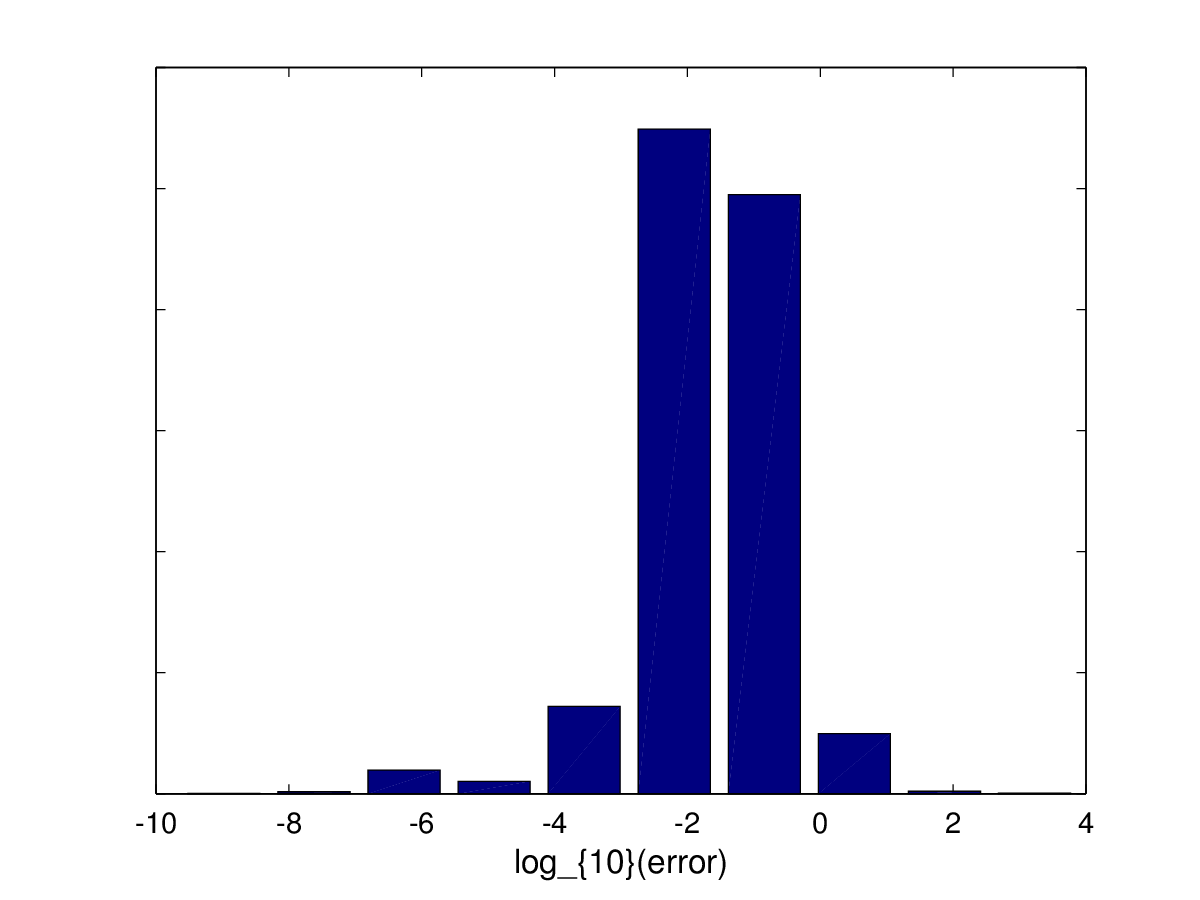
\includegraphics[width = \textwidth]{accHist.png}
%    \subcaption{Histogram of the absolute accuracy of the a.d. derivative}
%  \end{minipage}
%  \begin{minipage}[b]{.5\textwidth}
%    \centering
%    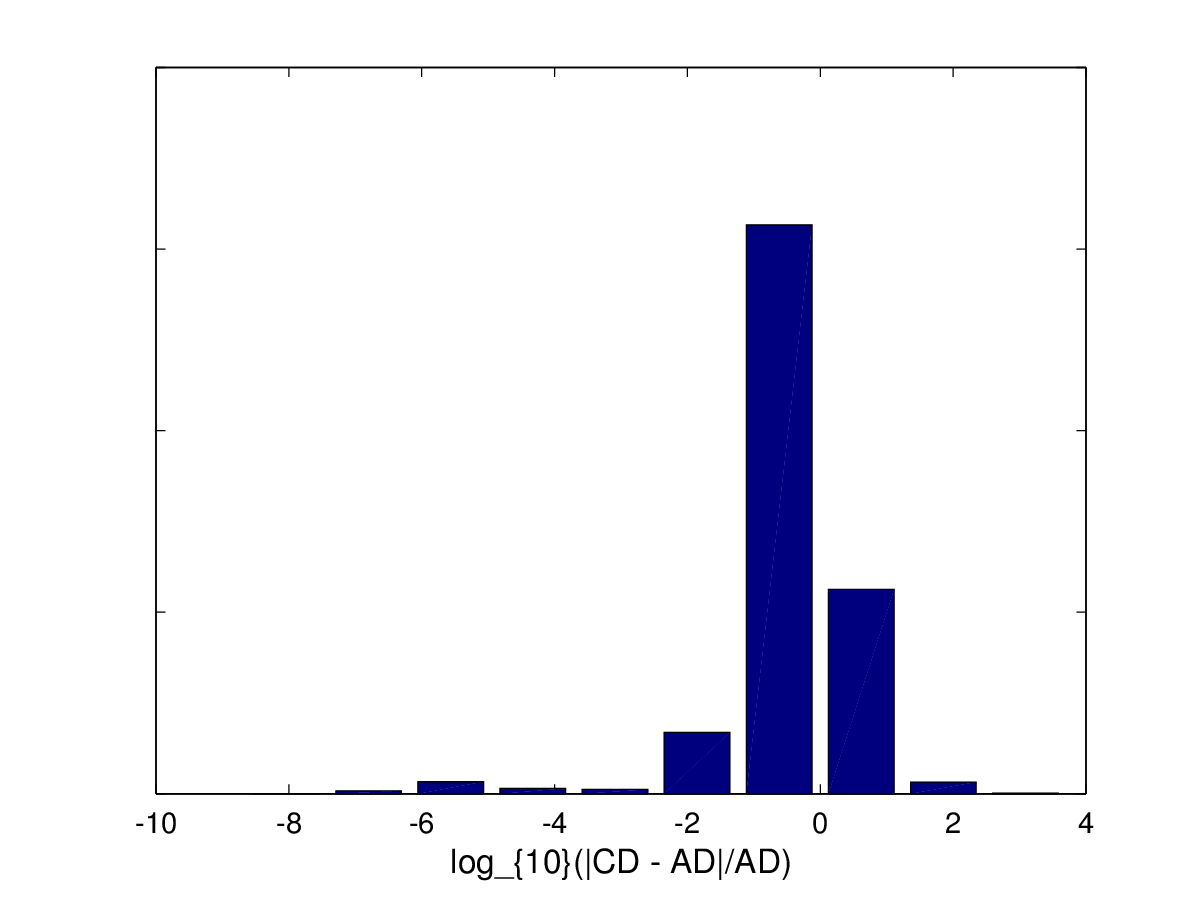
\includegraphics[width = \textwidth]{accHistRel.png}
%    \subcaption{Histogram of the relative accuracy of the a.d. derivative}
%  \end{minipage}
%\end{figure}
%
%This distribution 

\bibliographystyle{plain}
\bibliography{biblio}

\end{document}
